Qui viene riportato uno schema provvisorio creato dopo una prima analisi dei requisiti e dei concetti fondamentali. 
Nei paragrafi successivi le entità e le relazioni verranno raffinate e lo schema verrà corretto.\\

\begin{center}
\centerline{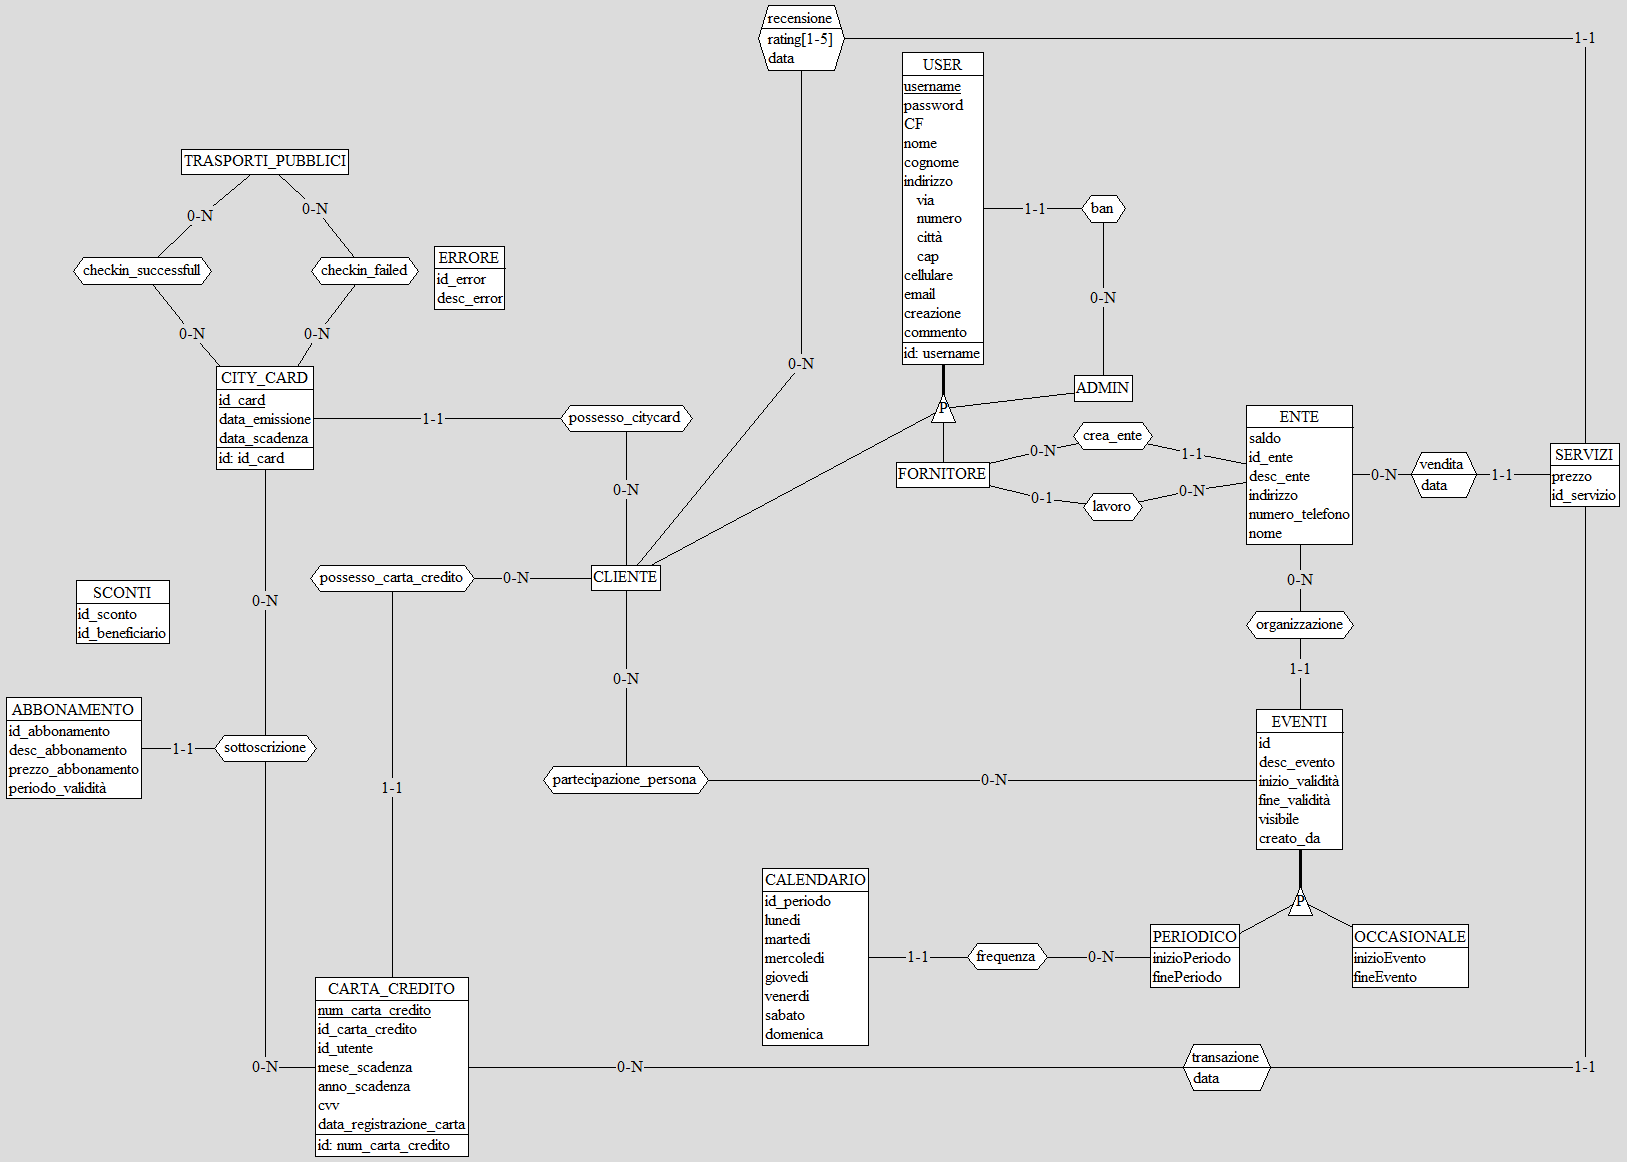
\includegraphics[width=0.9\paperwidth]{images/schema_ER_iniziale.png}}
\end{center}

\subsubsection{User}
\begin{center}
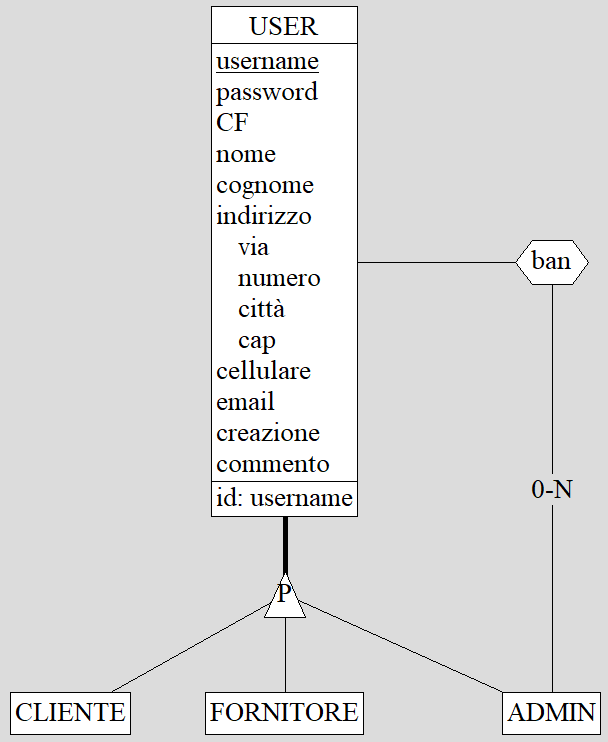
\includegraphics[width=0.95\columnwidth]{User.png}
\end{center}
I tre tipi di account che potranno essere creati, \textbf{CLIENTE}, \textbf{FORNITORE}, \textbf{ADMIN},  saranno sottocategorie di \textbf{USER}. Data la possibilità che una persona crei più di un account, ad esempio un fornitore vuole anche essere anche un cliente, l'identificazione avverrà tramite \textbf{username} e non il \textbf{CF}(codice fiscale).

\subsubsection{Ente}
\begin{center}
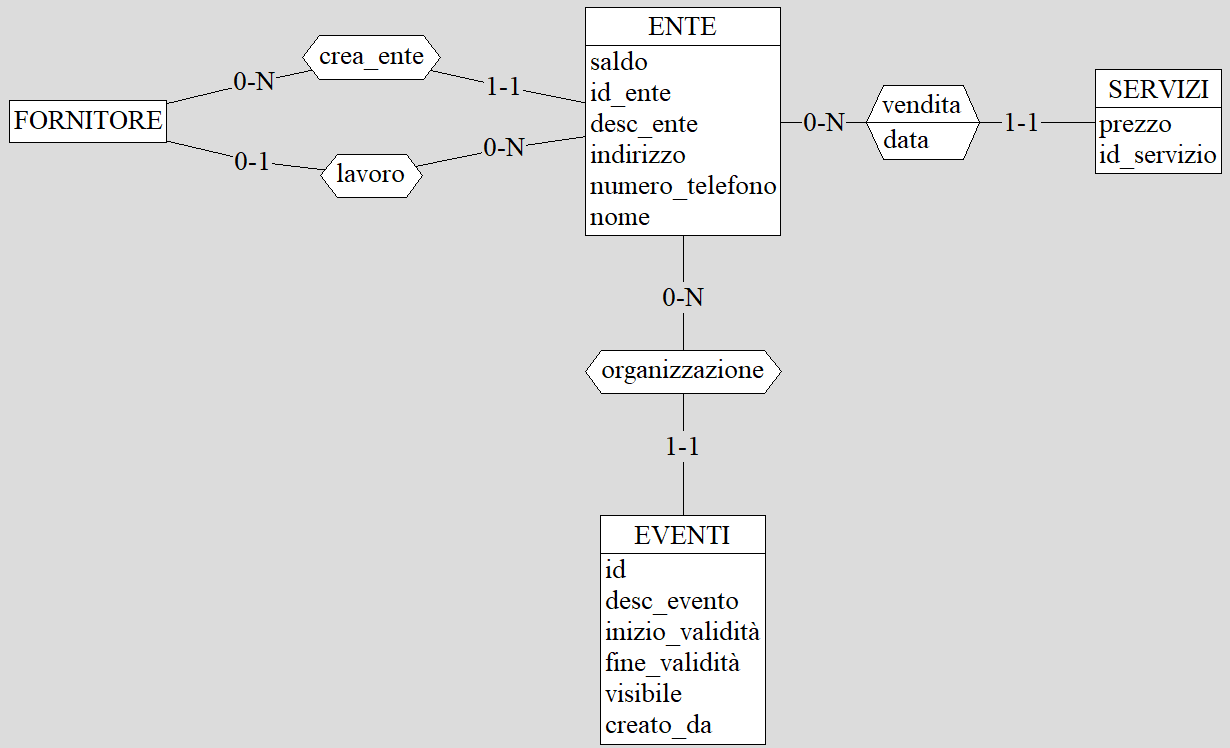
\includegraphics[width=0.95\columnwidth]{images/Ente.png}
\end{center}
L'ente è l'organizzazione che vende i servizi e organizza gli eventi. Possono venire creati dai fornitori. 
I fornitori possono associarsi ad un solo ente.


\subsubsection{Eventi}
\begin{center}
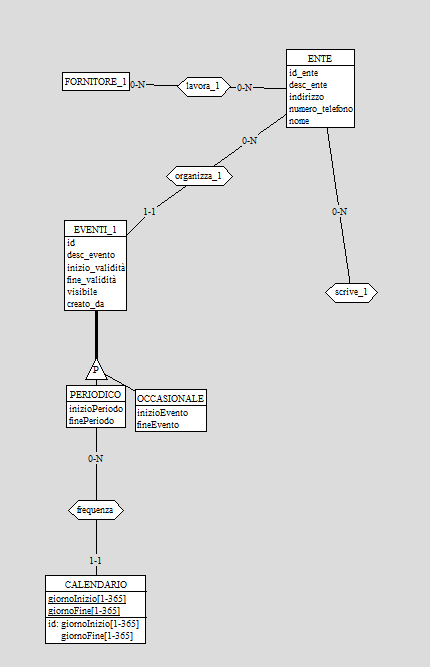
\includegraphics[width=0.95\columnwidth]{images/Eventi.png}
\end{center}
Gli eventi sono gli avvenimenti gratuiti accessibili dai clienti con prenotazione.
Sono organizzati dagli enti, un ente può organizzare più eventi ma un evento appartiene ad un solo ente.
Un evento può accadere in modalità periodica (ad esempio eventi a tema natalizio) oppure in modo occasionale (ad esempio inaugurazione di una nuova gelateria in centro).


\subsubsection{Servizi}
\begin{center}
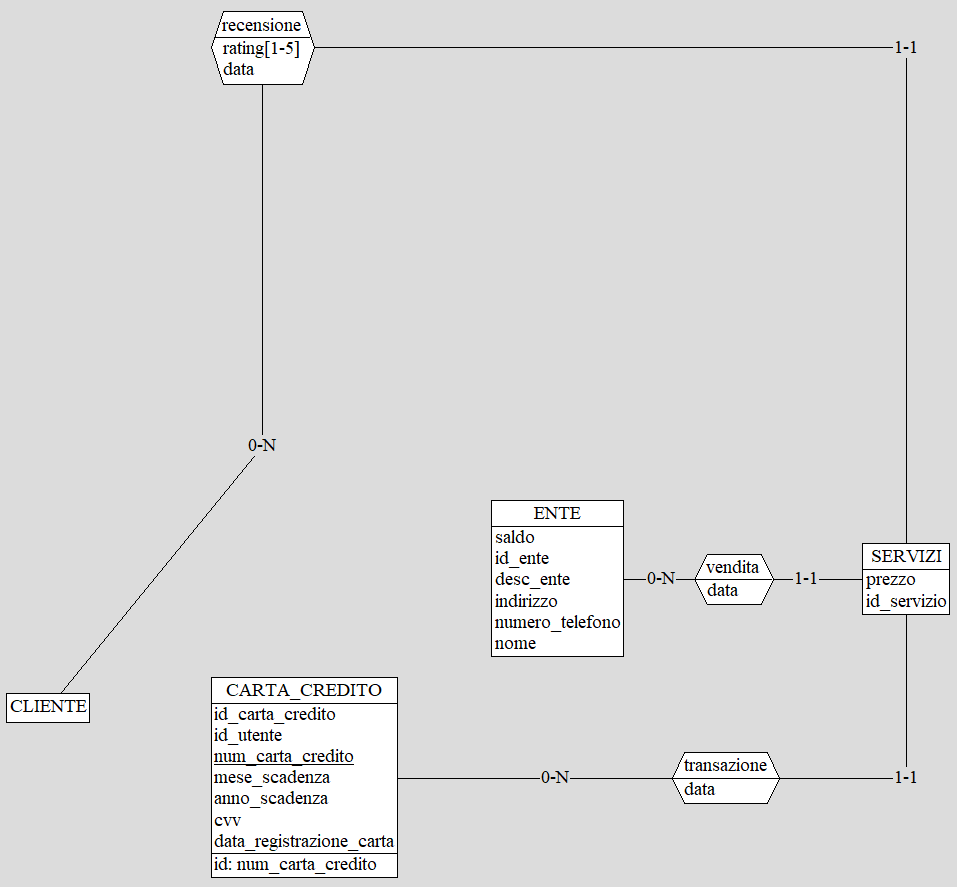
\includegraphics[width=0.95\columnwidth]{images/Servizi.png}
\end{center}
I servizi sono prodotti a pagamento accessibili dai clienti.
Sono venduti dagli enti, comprati tramite carta di credito e recensiti dai clienti dopo l'acquisto.


\subsubsection{CityCard}
\begin{center}
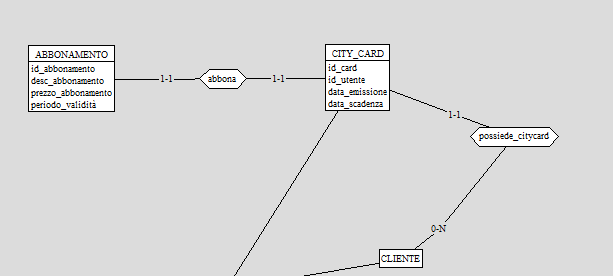
\includegraphics[width=0.95\columnwidth]{images/CityCard.png}
\end{center}
Ogni cliente può ottenere una CityCard che permetterà l'utilizzo gratuito dei mezzi pubblici e la prenotazione e l'acquisto di servizi forniti dagli enti. Per attivare la CityCard sarà necessario sottoscrivere ad un abbonamento a scelta tra tre diverse durate, dalla scelta fatta varierà la percentuale degli sconti applicati sui costi dei servizi.

\subsubsection{Trasporti Pubblici}
Si suppone che i trasporti pubblici siano una o più API esterne fornite dalla regione e/o da privati. Verrà creata una tabella con gli attributi minimali per imitarne la funzionalità. 


\subsubsection{Carta di credito}
\begin{center}
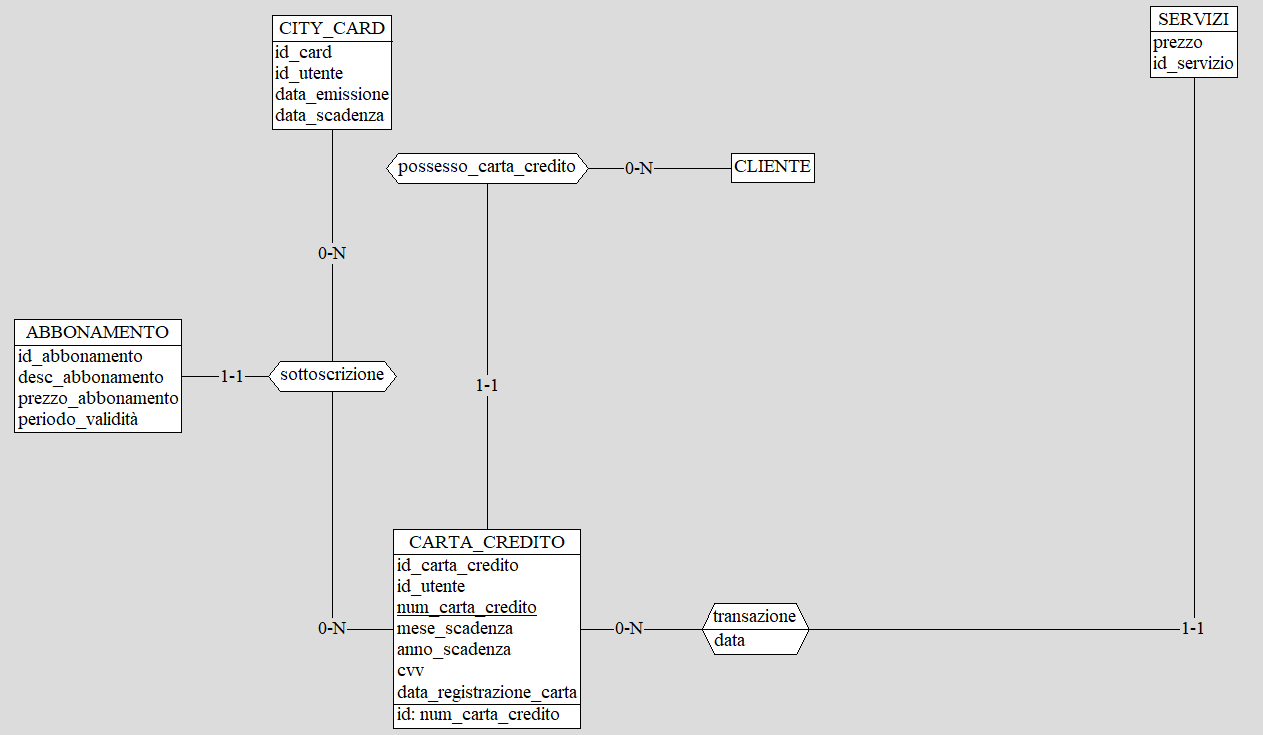
\includegraphics[width=0.95\columnwidth]{images/CartaDiCredito.png}
\end{center}
Ogni cliente, tramite la carta di credito, potrà acquistare l'abbonamento per la city card e pagare gli enti che forniscono i servizi.


\subsubsection{Abbonamento}
\begin{center}
\includegraphics[width=0.95\columnwidth]{images/Abbonamento.png}
\end{center}
L'abbonamento è lo strumento che permette l'attivazione della city card e, di conseguenza, l'acquisto di servizi. Ogni abbonamento ha una sua fascia con prezzo, durata e percentuale di sconto diversi, l'utente potrà scegliere quale acquistare. A prescindere dalla tipologia ogni abbonamento ha un periodo di validità.

\subsubsection{Sconti}
Lo sconto si caratterizza per la percentuale di riduzione di prezzo applicata ai servizi.